\section{FTS errors categorization} \label{sec:pipeline}

The pipeline illustrated in this work comprises an initial pre-processing step followed by the \textit{vectorization}, \textit{clustering} and \textit{description} stages.
Although conceptually similar to the workflow described in \citeA{clusterlog2021}, our approach considers some substantial modifications concerning mainly the pre-processing and the clustering stages.
Indeed, we apply minimal pre-processing to limit hard-coded feature engineering and let the vectorization stage figure out linguistic features of the error messages -- e.g. grammar, syntax, lexicon and semantic -- on its own.
The rationale behind this choice is that the resulting representation should be more expressive, thus better modeling the semantic of the messages and easing the successive clustering phase.

The next subsections provide a thorough description of each stage of our pipeline.


% Although the workflow in
% \citeA{clusterlog2021} accounts for all these phases and could be adapted for FTS errors as is, it also presents some relevant drawbacks.
% First, the pre-processing and vectorization stages reduce all the principal sources of variability, turning the whole approach into something close to unique strings grouping (assuming a smart and flexible definition of unique strings). 
% For example,  the raw error messages are transformed into structured templates where the same placeholder replaces all parametric parts.
% This choice drastically decreases the data variability. Also, it hampers the usage of parameter values for error discrimination, potentially masking faults due to specific components, e.g. one particular file is corrupted and needs restoration, or a determined site/service is not responding.
% Moreover, performing principal components decomposition on the word2vec embedding further reduces the expressive power of the learned representation.
% Although the previous strategies are crucial to comply with the runtime and computing requirements of particular use cases, they seem to contrast the current best practices for text processing. 
% In fact,  the recent applications in NLP literature suggest exploiting the increased computing power of modern architectures to train bigger models with minimal hard-coded feature engineering. 
% The idea behind that is to let the model figure out linguistic features -- e.g. grammar, syntax, lexicon and semantic -- and relations among tokens, thus endowing the resulting model with increased expressive power.
% As a result, the previous strategies likely hinder learning an optimal embedding, perhaps questioning the need for the word2vec language model for text vectorization in the first place.
% Another drawback is that no auxiliary information concerning the transfer processes is considered alongside the error message. This potentially prevents the system from spotting higher-level correlations with transfer features not contained in the error string.

% In order to mitigate these limitations, our approach considers some major modifications concerning mainly the pre-processing and the clustering stages.
% The next subsections provide a thorough description of each step of our workflow.% and describe the main differences with respect to the alternatives.

\sidenote[Luca][notesyellow]{aggiungere schema pipeline: prendere dalle varie slide + google draw}

\begin{figure}
    \centering
    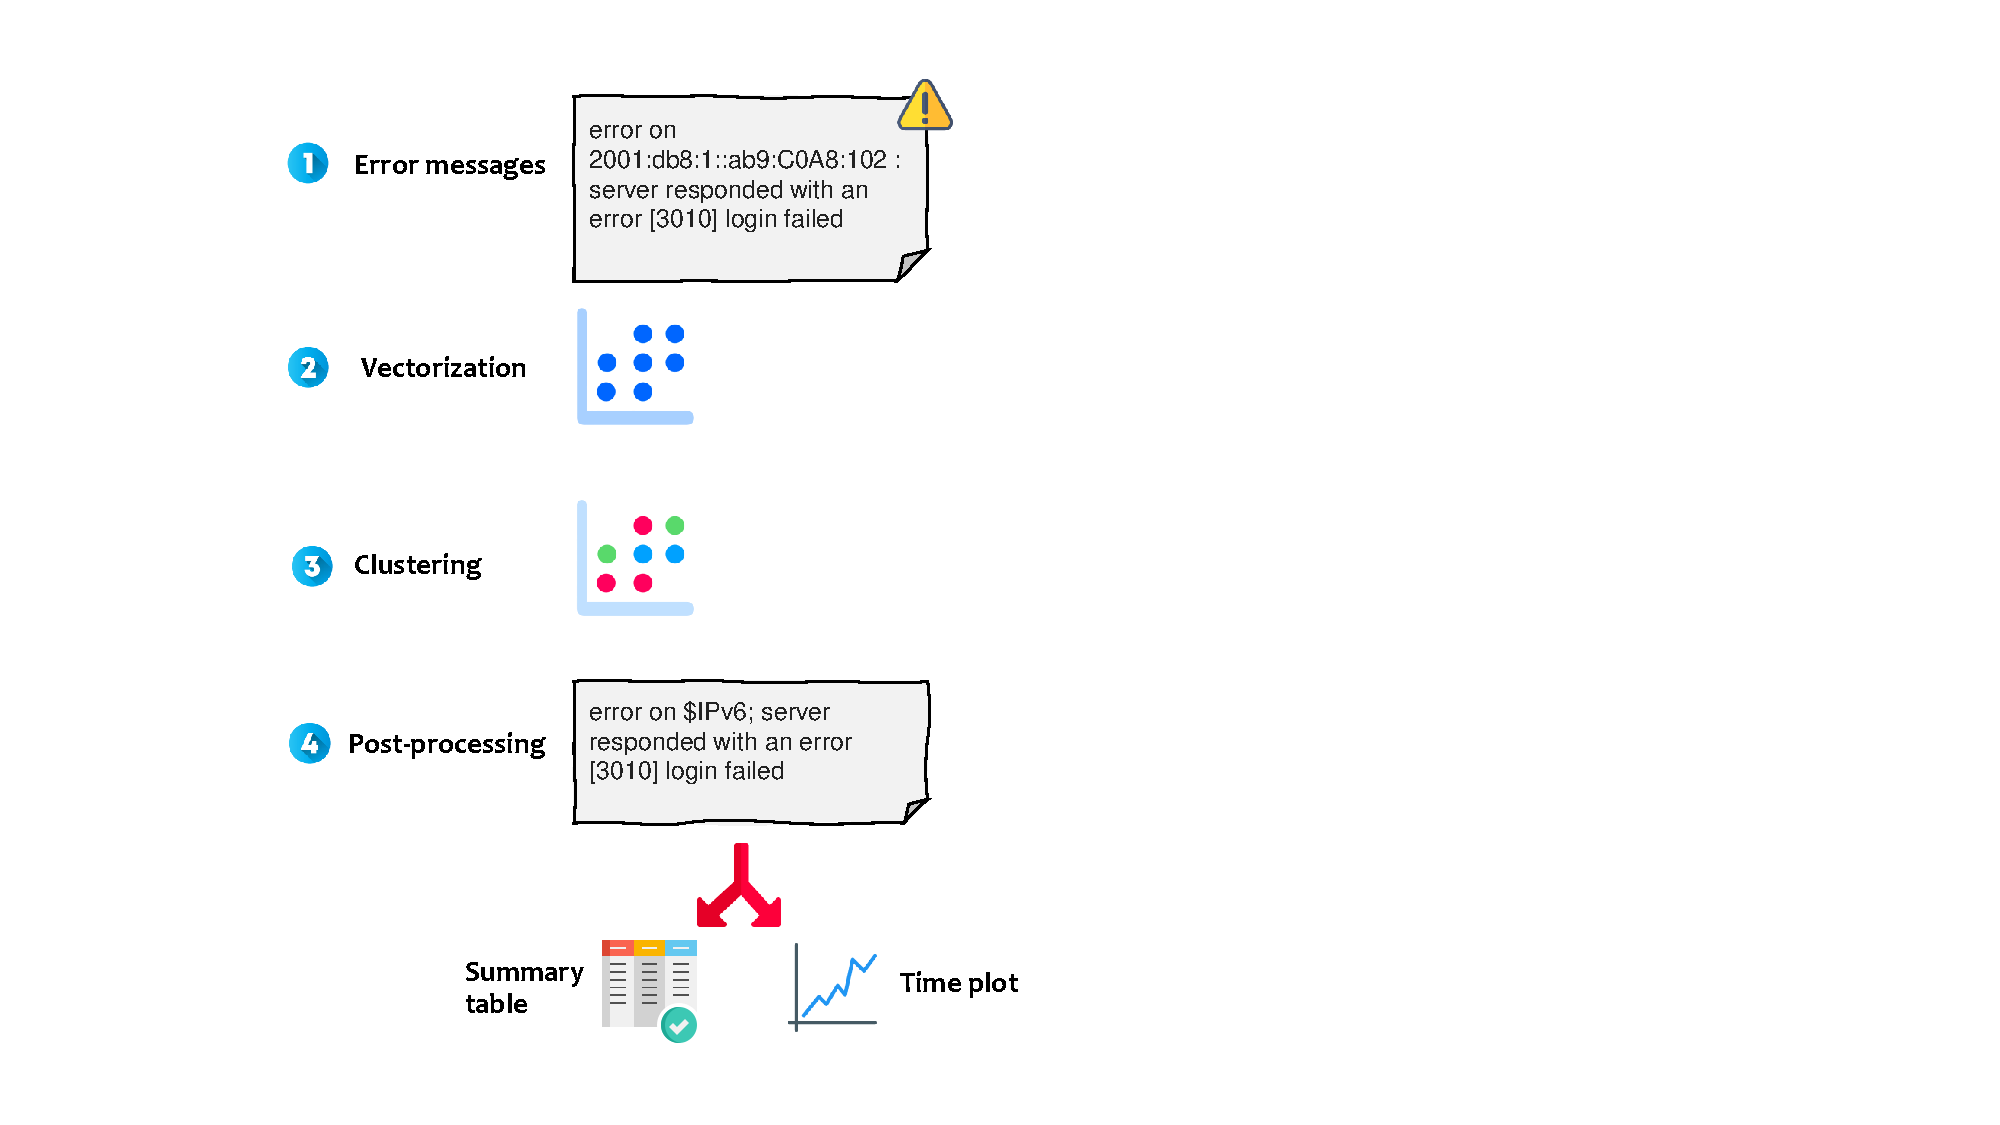
\includegraphics[width=.5\textwidth]{figures/410_method/pipeline.pdf}
    \caption{Caption}
    \label{fig:my_label}
\end{figure}

\subsection{Pre-processing}

% Of course, the string format of the raw data is highly unstructured and impractical to handle, thus limiting the plethora of applicable techniques. 
% For this reason, the (possibly long) strings incorporated in the documents are first quantized into unitary pieces of textual information, tokens, from which the raw strings can be reconstructed. These process may vary from simply using words \cite{bengio2003word, mccann2017word} or characters \cite{ling2015char, dhingra2016char}, to more complex strategies involving subwords \cite{gage1994subword, sennrich2016subword}, sentences \cite{kiros2015sentence}, documents \cite{le2014documents} and topics \cite{niu2015topic}. 

The pre-processing phase is crucial to any data analysis workflow. Various best practices are suggested for data cleaning, and custom feature engineering is often adopted to feed models with the most relevant information in the most suitable format.
Our approach tries to limit these elaborations to the bare minimum to avoid injecting too much prior knowledge into the system and probe the model's ability to learn by itself.
The resulting pipeline is described below and summarized in \cref{tab:preproc-pipeline}.

As a first step, the raw error strings are transformed to lowercase and enriched by appending the source and destination hostnames. In particular, both hostnames are inserted at the end of each message with prepended \textbox{src\_} or \textbox{dst\_} prefixes to distinguish whether they were involved as source or destination, respectively.
The resulting text then undergoes a process of quantization whereby the raw strings are decomposed into unitary pieces of information.
This process is commonly referred to as tokenization and the resulting atomic units are called tokens. Various approaches have been proposed in the literature ranging from simply using words \cite{bengio2003word, mccann2017word} or characters \cite{ling2015char, dhingra2016char}, to more complex strategies involving subwords \cite{gage1994subword, sennrich2016subword}, sentences \cite{kiros2015sentence}, documents \cite{le2014documents} and topics \cite{niu2015topic}. 
In our case, we resort to whitespace tokenization for the sake of simplicity, which means individual words are used as tokens.
Once tokens are obtained, they are stripped of leading and trailing punctuation \mbox{(\textbox{":;,.-"})}% (\textbox{``:", ``;", ``,", ``.", ``-"})%(\textbox{":;,.- "})
.
After that, tokens corresponding to common English stopwords\footnote{refer to \texttt{pyspark.ml.feature.StopWordsRemover} documentation for a full list} or unuseful punctuation \mbox{(\textbox{":-+"})} %(\textbox{[``:", ``-", ``+"]}) 
are discarded.
Finally, the URL addresses are split into two components: the net location and the relative path of the requested resources. For instance, 
\textbox{httpg://<hostname>:<port>:/srm/managerv2} is decomposed as \textbox{httpg://<hostname>:<port>} and \textbox{srm/managerv2}%
% \textbox{httpg://tbn18.nikhef.nl:8446:/srm/managerv2} is decomposed as \textbox{httpg://tbn18.nikhef.nl:8446} and \textbox{srm/managerv2}
.
In this way, it is possible to exploit the compositional structure of the URL addresses to reduce the vocabulary of unique tokens. Also, this allows the model to disentangle the contribution of the single parts in different messages.

\begin{table} \scriptsize
\begin{tabular}{p{1.9cm} | p{12cm}}
\textbf{raw message} &
  ``DESTINATION OVERWRITE srm-ifce err: Communication error on send, err:  {[}SE{]}{[}srmRm{]}{[}{]} httpg://hostname01.Site-4.ch:8443/srm/managerv2:  CGSI-gSOAP running on fts-address-004.cern.ch reports Error initializing  context GSS Major Status: Authentication Failed  GSS Minor Status Error  Chain: globus\_gsi\_gssapi: SSL handshake problems  globus\_gsi\_callback\_module: Could not verify credential  globus\_gsi\_callback\_module: Could not verify credential  globus\_gsi\_callback\_module: The certificate has been revoked: Serial  number = -1 (0xFFFFFFFFFFF" \\[0.2cm]
\textbf{append hostnames} &
   ``DESTINATION OVERWRITE srm-ifce err: Communication error on send, err:  {[}SE{]}{[}srmRm{]}{[}{]} httpg://hostname01.Site-4.ch:8443/srm/managerv2:  CGSI-gSOAP running on fts-address-004.cern.ch reports Error initializing  context GSS Major Status: Authentication Failed  GSS Minor Status Error  Chain: globus\_gsi\_gssapi: SSL handshake problems  globus\_gsi\_callback\_module: Could not verify credential  globus\_gsi\_callback\_module: Could not verify credential  globus\_gsi\_callback\_module: The certificate has been revoked: Serial  number = -1 (0xFFFFFFFFFFF src\_srmatlas.pic.es dst\_hostname01.Site-4.ch" \\[0.2cm]
\textbf{tokenization} &
   {[}``destination", ``overwrite", ``srm-ifce", ``err:", ``communication", ``error", ``on", ``send,", ``err:", ``{[}se{]}{[}srmrm{]}{[}{]}", ``httpg://hostname01.Site-4.ch:8443:/srm/managerv2:", ``gsi-gsoap", ``running", ``on", ``fts-atlas-005.cern.ch", ``reports", ``error", ``initializing", ``context", ``gss", ``major", ``status:", ``authentication", ``failed", ``gss", ``minor", ``status", ``error", ``chain:", ``globus\_gsi\_gssapi:", ``ssl", ``handshake", ``problems", ``globus\_gsi\_callback\_module:", ``could", ``not", ``verify", ``credential", ``globus\_gsi\_callback\_module:", ``could", ``not", ``verify", ``credential", ``globus\_gsi\_callback\_module:", ``the", ``certificate", ``has", ``been", ``revoked:", ``serial", ``number", ``=", ``-1", ``(0xfffffffffff", ``src\_srmatlas.pic.es", ``dst\_hostname01.Site-4.ch"{]} \\[0.2cm]
\textbf{remove punctuation} &
  {[}``destination", ``overwrite", ``srm-ifce", ``err", ``communication", ``error", ``on", ``send", ``err", ``{[}se{]}{[}srmrm{]}{[}{]}", ``httpg://hostname01.Site-4.ch:8443:/srm/managerv2", ``cgsi-gsoap", ``running", ``on", ``fts-atlas-005.cern.ch", ``reports", ``error", ``initializing", ``context", ``gss", ``major", ``status", ``authentication", ``failed", ``gss", ``minor", ``status", ``error", ``chain", ``globus\_gsi\_gssapi", ``ssl", ``handshake", ``problems", ``globus\_gsi\_callback\_module", ``could", ``not", ``verify", ``credential", ``globus\_gsi\_callback\_module", ``could", ``not", ``verify", ``credential", ``globus\_gsi\_callback\_module", ``the", ``certificate", ``has", ``been", ``revoked", ``serial", ``number", ``=", ``1", ``(0xfffffffffff", ``src\_srmatlas.pic.es", ``dst\_hostname01.Site-4.ch"{]} \\[0.2cm]
\textbf{remove stopwords} &
  {[}``destination", ``overwrite", ``srm-ifce", ``err", ``communication", ``error", ``send", ``err", ``{[}se{]}{[}srmrm{]}{[}{]}", ``httpg://hostname01.Site-4.ch:8443:/srm/managerv2,cgsi-gsoap", ``running", ``fts-atlas-005.cern.ch", ``reports", ``error", ``initializing", ``context", ``gss", ``major", ``status", ``authentication", ``failed", ``gss", ``minor", ``status", ``error", ``chain", ``globus\_gsi\_gssapi", ``ssl", ``handshake", ``problems", ``globus\_gsi\_callback\_module", ``verify", ``credential", ``globus\_gsi\_callback\_module", ``verify", ``credential", ``globus\_gsi\_callback\_module", ``certificate", ``revoked", ``serial", ``number", ``=", ``1", ``(0xfffffffffff", ``src\_srmatlas.pic.es", ``dst\_hostname01.Site-4.ch"{]} \\[0.2cm]
\textbf{url split} &
  {[}``destination", ``overwrite", ``srm-ifce", ``err", ``communication", ``error", ``send", ``err", ``{[}se{]}{[}srmrm{]}{[}{]}", ``httpg://hostname01.Site-4.ch:8443", ``/srm/managerv2", ``cgsi-gsoap", ``running", ``fts-atlas-005.cern.ch", ``reports", ``error", ``initializing", ``context", ``gss", ``major", ``status", ``authentication", ``failed", ``gss", ``minor", ``status", ``error", ``chain", ``globus\_gsi\_gssapi", ``ssl", ``handshake", ``problems", ``globus\_gsi\_callback\_module", ``verify", ``credential", ``globus\_gsi\_callback\_module", ``verify", ``credential", ``globus\_gsi\_callback\_module", ``certificate", ``revoked", ``serial", ``number", ``=", ``1", ``(0xfffffffffff", ``src\_srmatlas.pic.es", ``dst\_hostname01.Site-4.ch"{]}
\end{tabular}
\caption{\textbf{Message pre-processing pipeline.} The table illustrates the \mbox{pre-processing} steps (left) and the resulting data (right) for a sample error message. The raw error string is reported at the top, and the resulting pre-processed data at the bottom}
\label{tab:preproc-pipeline}
\end{table}



\subsection{Vectorization} \label{sec:vectorization}

%The vectorization stage transforms the pre-processed text of each error message into numeric information that quantitative techniques can digest.
%In particular, we leverage the \textbf{word2vec} language model \cite{mikolov2013word2vec} to compute token embeddings.
In the vectorization stage we leverage the \textbf{word2vec} language model \cite{mikolov2013word2vec} to compute message embeddings starting from pre-processed tokens.
Although more recent and powerful alternatives as the ones described in \cref{sec:related_opint} are available, they do not work well with short-text data \cite{albalawi2020short-text}. Thus, the simpler yet effective word2vec model is used here.

The idea behind word2vec is to find a convenient mapping between tokens (words) and a vectorial space where token linguistic relations are preserved, thus producing a distributed representation of words.
In this way, we obtain a numerical representation of textual data that quantitative algorithms can further process.
In particular, two alternative implementations of the word2vec model are available (see \cref{fig:word2vec}).
Both alternatives are based on a shallow (2-layer) neural network architecture and use a sliding window (context) of fixed size, $w$, around the current word, $w_t$.
The continuous bag-of-words (CBOW) model sets the learning objective to predict the current word from the surrounding context.
Conversely, the \mbox{skip-gram} model tries to guess the terms present in the context window starting from the current word.
To achieve that, the input words are first represented as 1-hot vectors of size $V$, where $V$ is the number of terms present in the corpus (vocabulary size). 
During this encoding step, a minimum allowed token frequency, $min\_count$ is set to discard terms appearing less than such threshold. This trick limits the vocabulary size by excluding rare tokens, thus lowering the computational requirements.
These input vectors pass through the first layer that projects them to a hidden space of customizable dimension, $h$. This mapping (embedding) is learned during the training phase such that terms often used together or in similar contexts should be projected nearby.
Finally, the resulting representations are put through the next network layer to get the predicted context (in the case of CBOW) or current words (skip-gram).

This work adopts the word2vec version exploiting the skip-gram architecture and uses its \texttt{pyspark} implementation.
Specifically, the model is trained on one month of data from 2020-10-01 to 2020-10-31.
In total, nearly 28.6 M error messages are analyzed, corresponding to a vocabulary of 970 unique tokens.
Once the model is trained, the resulting word embeddings are used to transform single tokens into numerical vectors, and they are then averaged to get the corresponding message representations.
Regarding hyper-parameters, the window size, the embedding size and the minimum count were the ones affecting the final representation the most.
For this reason, a grid-search is conducted to compare alternative parametrizations.  
The optimal configuration is then chosen based on the compactness of the resulting groups in the following clustering stage.
Specifically, the values of $w=12$, $h=300$ and $min\_count=50$ seem to work best in our use case.

\begin{figure}
    \centering
    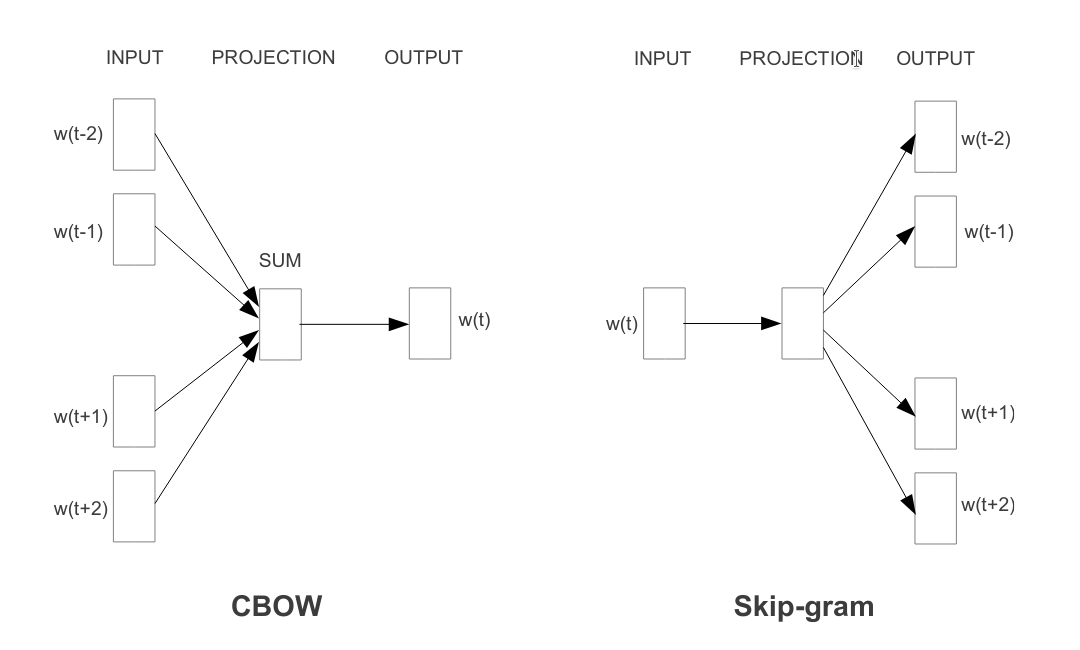
\includegraphics[width=\textwidth]{figures/410_method/word2vec.png}
    \caption{\textbf{Word2vec model architectures.} The CBOW architecture predicts the current word based on the
context, and the Skip-gram predicts surrounding words given the current word. The figure is borrowed from the original paper \protect \cite{mikolov2013word2vec}
}
    \label{fig:word2vec}
\end{figure}
\subsection{Clustering} \label{sec:clustering}

The next step of the pipeline is the clustering stage.
Cluster analysis examines the task of grouping a set of objects based on a given measure of distance or similarity.
This is a well-studied topic typically conducted to discover underlying structures in data during exploratory analysis or pattern recognition.

One of the most intuitive and widely adopted strategies to tackle this problem is the so-called \textit{k-means} algorithm \cite{lloyd1982kmeans}.
This technique is an iterative local search solution, and it refers to a particular formulation of the problem where the number of output groups, $k$, is supposedly known.
The algorithm evolves in four simple steps, starting from this prior information and after establishing a suitable distance measure to express the similarity between data points.
\Cref{fig:kmeans-pipeline} summarizes the k-means pipeline from raw data to the final clusters discovered applied to some toy data points.
In the initialization phase, $k$ arbitrary centers (also named \textit{centroids}) are chosen uniformly at random from the data points (\cref{fig:kmeans-pipeline:init}). 
In the next step, the data are split into clusters by mapping each data point to the nearest center (\cref{fig:kmeans-pipeline:updateClusters}). 
Once the groups are formed, the centroids are re-computed as the center of mass of all points assigned to the corresponding cluster (\cref{fig:kmeans-pipeline:updateCentroids}).
Finally, the last two steps are repeated until a convergence criterion is met (\cref{fig:kmeans-pipeline:result}).
% \Cref{fig:kmeans-pipeline} illustrates an animation of the first iteration and the final result of the algorithm described above applied to some toy data points.

% \begin{figure}
%     \centering
%     \subfloat[raw data]{
%     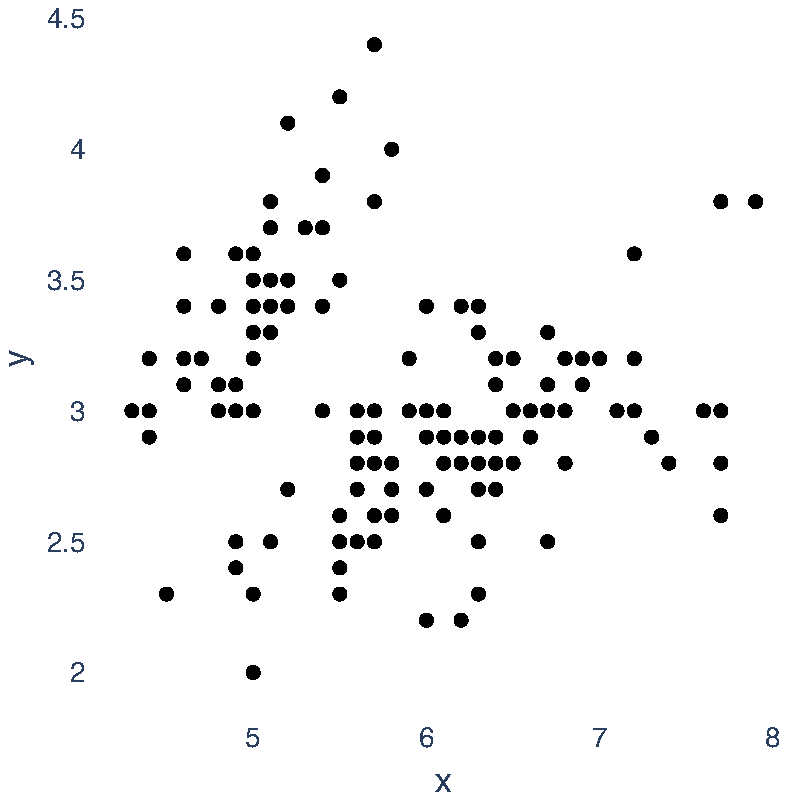
\includegraphics[width=0.5\textwidth]{figures/410_method/kmeans/kmeans_data.pdf}
%     }
%     \subfloat[initialization]{
%     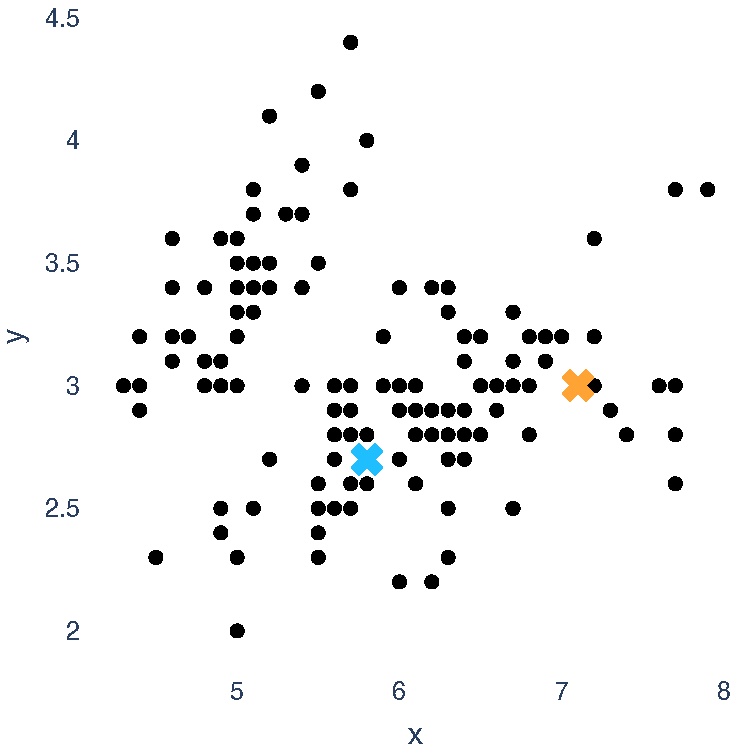
\includegraphics[width=0.5\textwidth]{figures/410_method/kmeans/kmeans_centroid2.pdf}
%     }
    
%     \subfloat[update clusters]{
%     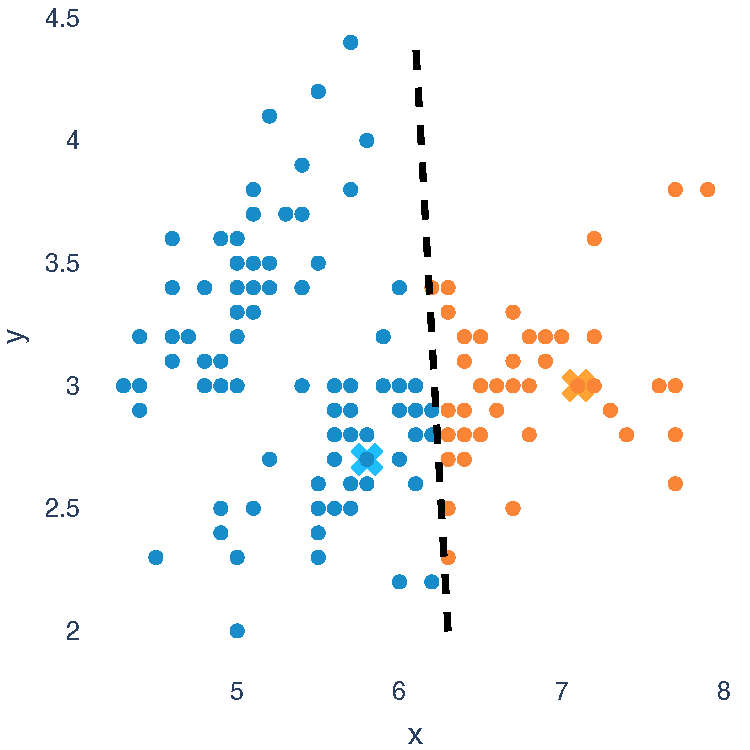
\includegraphics[width=0.5\textwidth]{figures/410_method/kmeans/kmeans_updateCluster.pdf}
%     }
%     \subfloat[update centroids]{
%     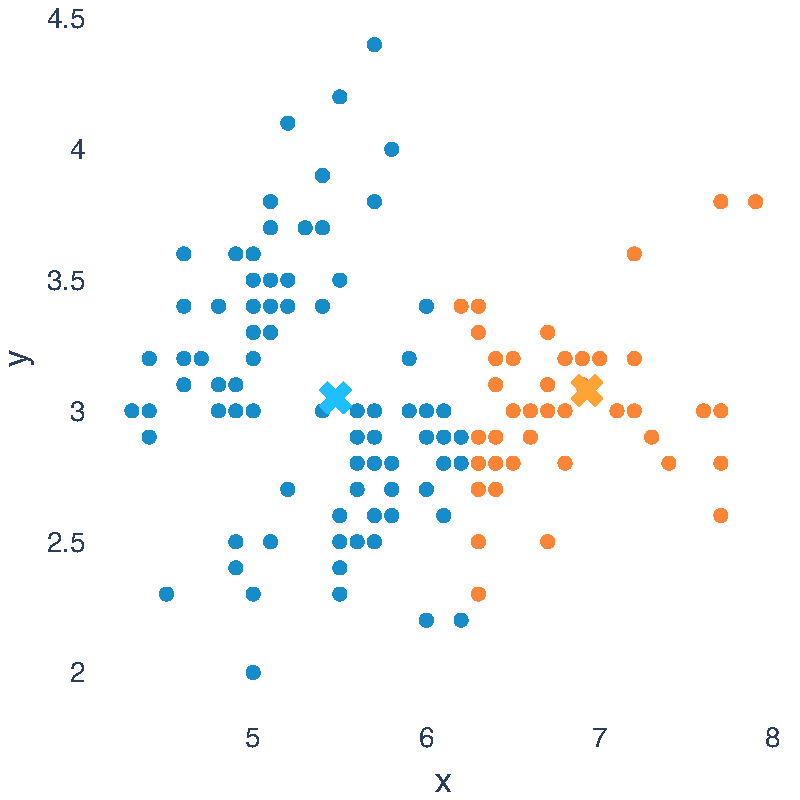
\includegraphics[width=0.5\textwidth]{figures/410_method/kmeans/kmeans_updateCentroids.pdf}
%     }
%     \caption{\textbf{K-Means clustering.} The algorithm performs an iterative search by alternately grouping observations around cluster centers of mass and updating such centroids.}
%     \label{fig:kmeans-pipeline1}
% \end{figure}

% \begin{figure}
%     \centering
%     \subfloat[raw data]{
%     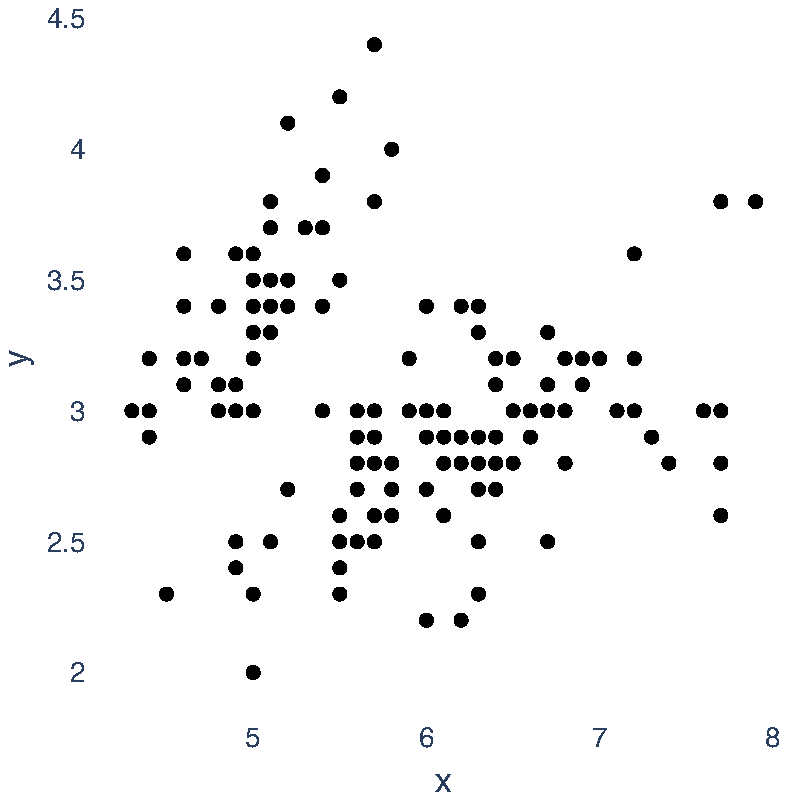
\includegraphics[width=0.4\textwidth]{figures/410_method/kmeans/kmeans_data.pdf}
%     }
%     \subfloat[final result]{
%     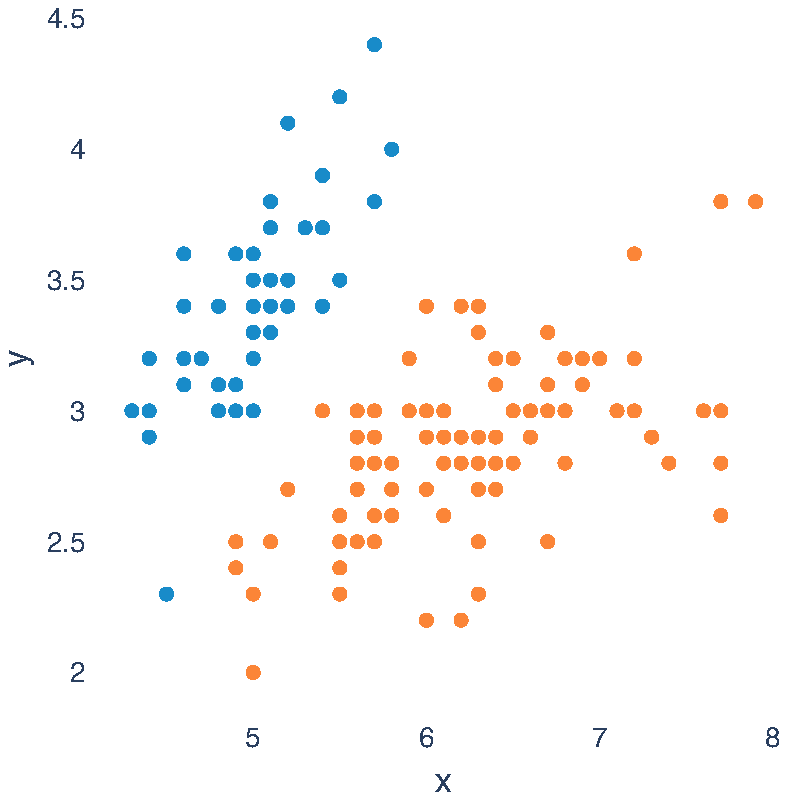
\includegraphics[width=0.4\textwidth]{figures/410_method/kmeans/kmeans_finalResult.pdf}
%     }
    
%     \subfloat[initialization first centroid]{
%     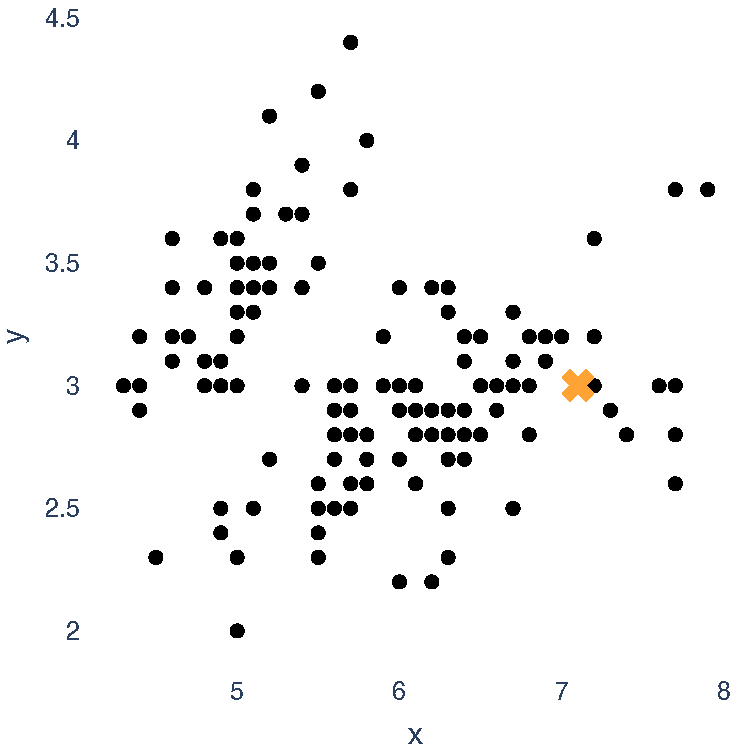
\includegraphics[width=0.4\textwidth]{figures/410_method/kmeans/kmeans_centroid1.pdf}
%     }
%     \subfloat[initialization second centroid]{
%     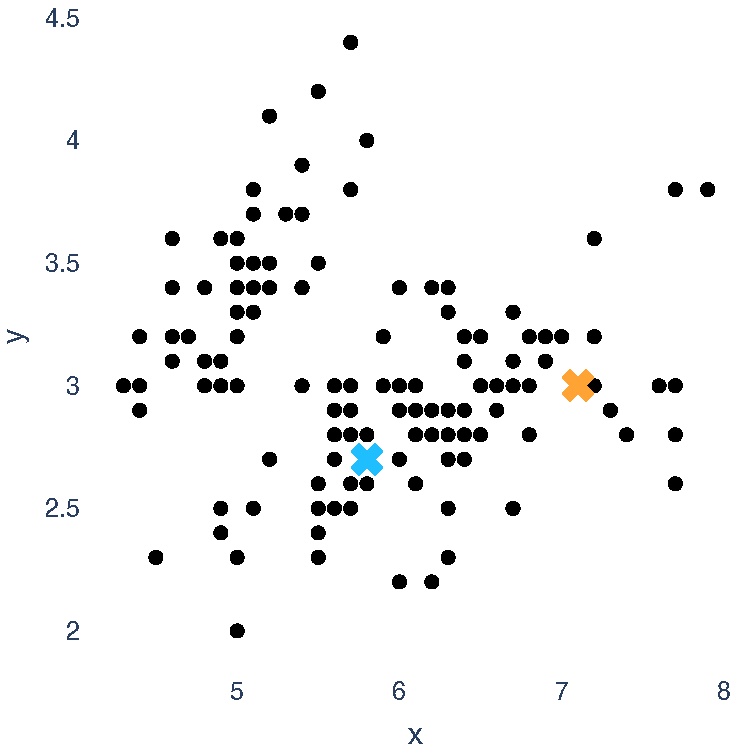
\includegraphics[width=0.4\textwidth]{figures/410_method/kmeans/kmeans_centroid2.pdf}
%     }
    
%     \subfloat[update clusters]{
%     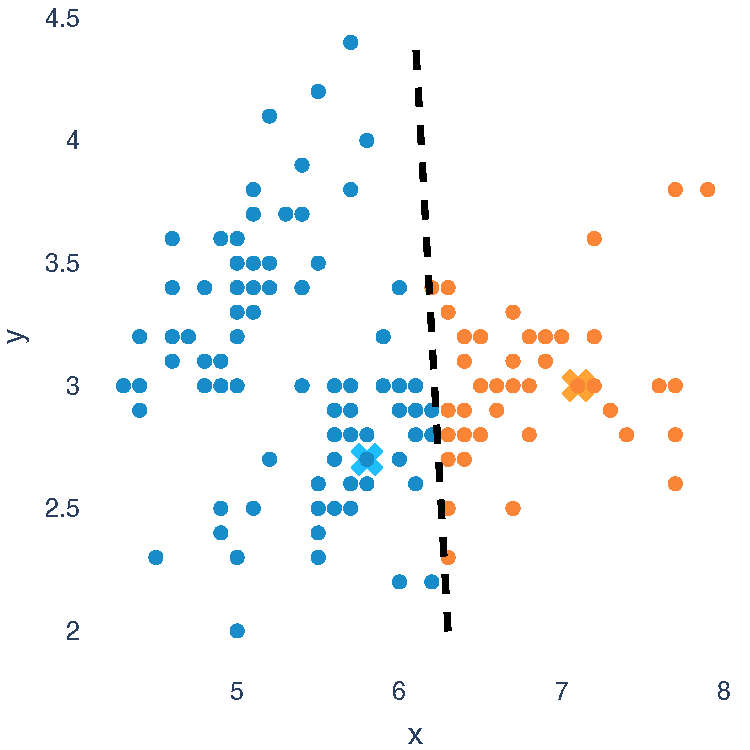
\includegraphics[width=0.4\textwidth]{figures/410_method/kmeans/kmeans_updateCluster.pdf}
%     }
%     \subfloat[update centroids]{
%     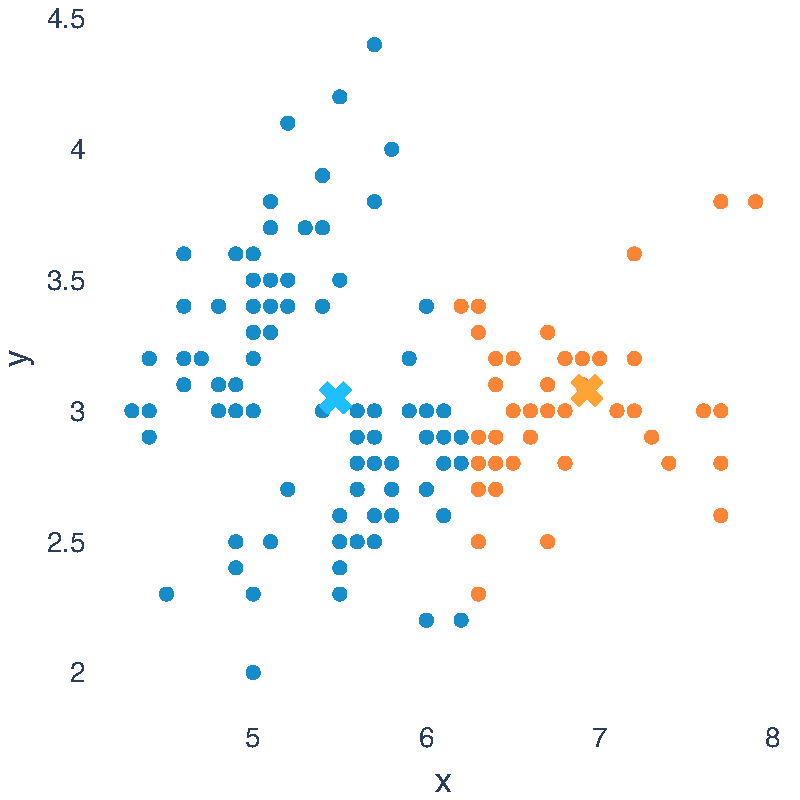
\includegraphics[width=0.4\textwidth]{figures/410_method/kmeans/kmeans_updateCentroids.pdf}
%     }
%     \caption{\textbf{K-Means clustering.} The algorithm performs an iterative search by alternately grouping observations around cluster centers and updating centroids.}
%     \label{fig:kmeans-pipeline1}
% \end{figure}

\begin{figure}
    \centering
    % \subfloat[raw data]{
    % 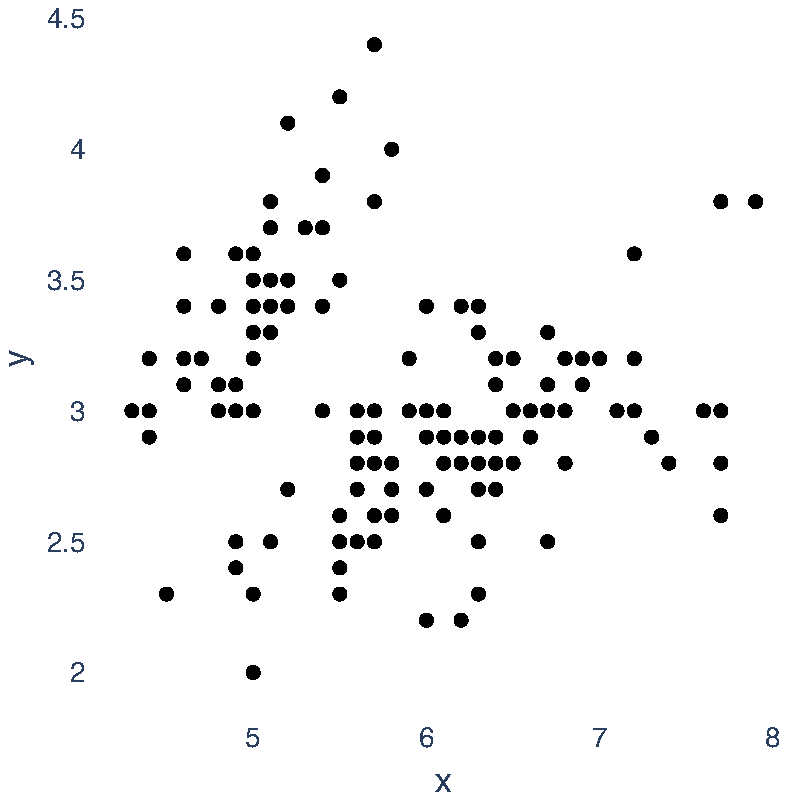
\includegraphics[width=0.5\textwidth]{figures/410_method/kmeans/kmeans_data.pdf}
    % }
    \subfloat[initialization]{
    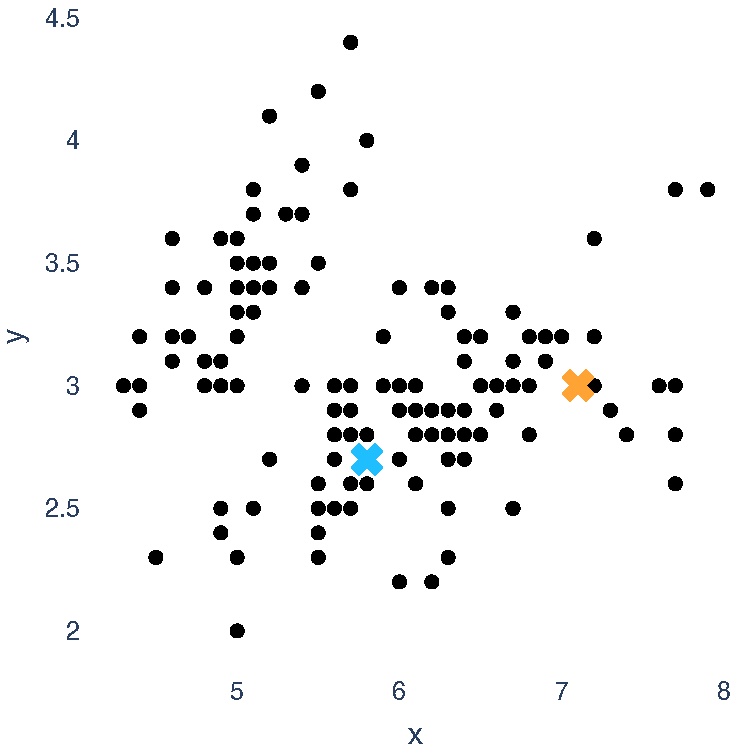
\includegraphics[width=0.5\textwidth]{figures/410_method/kmeans/kmeans_centroid2.pdf}\label{fig:kmeans-pipeline:init}
    }
    \subfloat[update clusters]{
    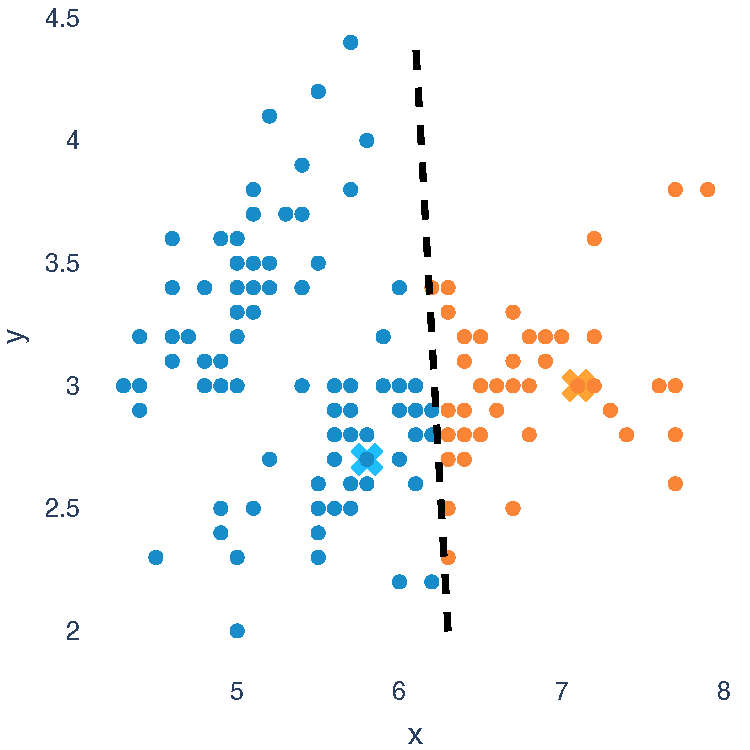
\includegraphics[width=0.5\textwidth]{figures/410_method/kmeans/kmeans_updateCluster.pdf}\label{fig:kmeans-pipeline:updateClusters}
    }
    
    \subfloat[update centroids]{
    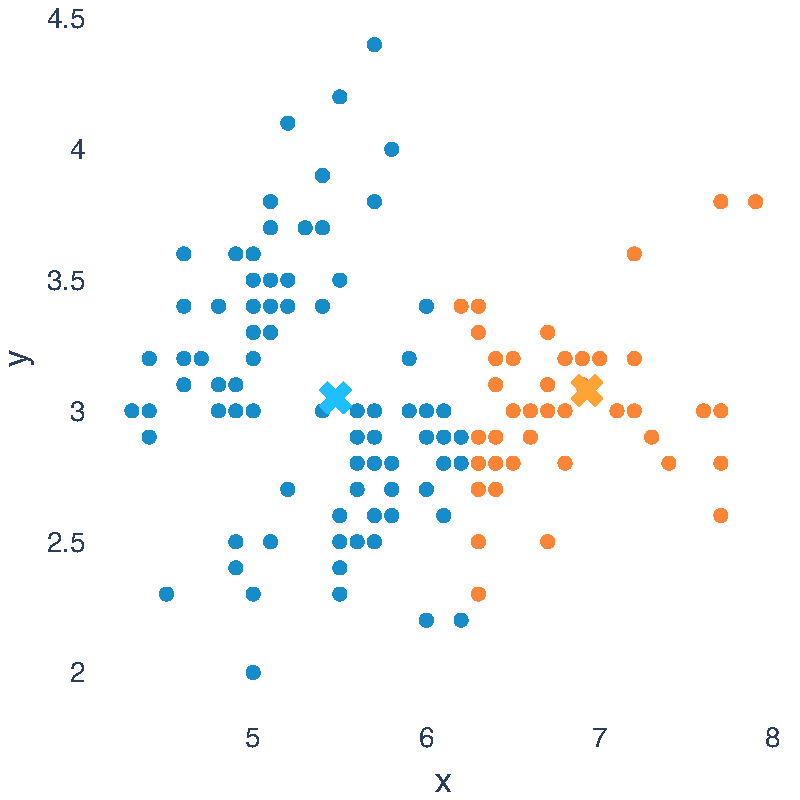
\includegraphics[width=0.5\textwidth]{figures/410_method/kmeans/kmeans_updateCentroids.pdf}\label{fig:kmeans-pipeline:updateCentroids}
    }
    \subfloat[final result]{
    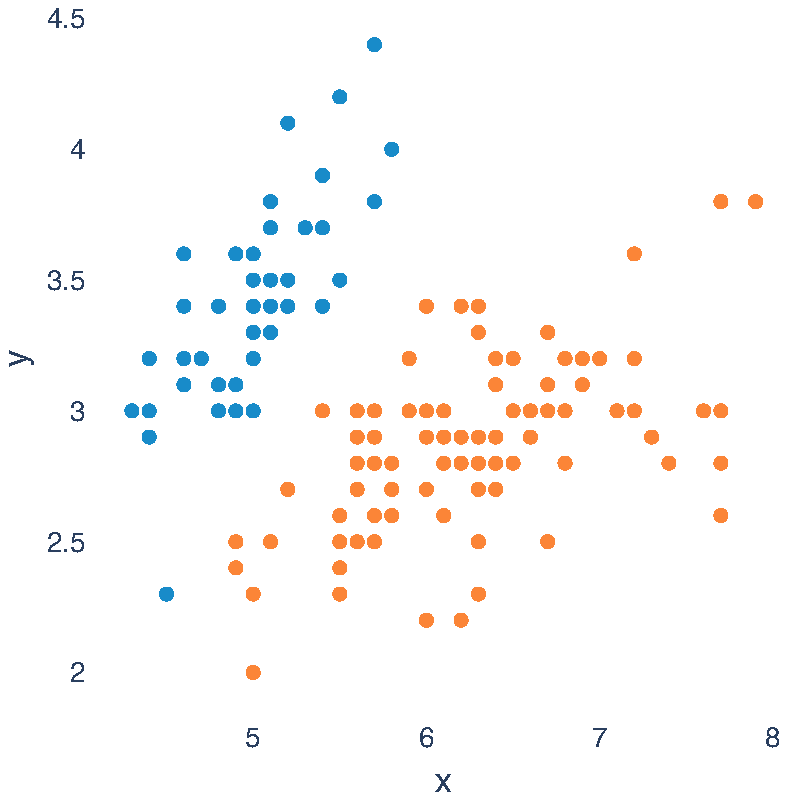
\includegraphics[width=0.5\textwidth]{figures/410_method/kmeans/kmeans_finalResult.pdf}\label{fig:kmeans-pipeline:result}
    }
    \caption{\textbf{K-Means clustering.} The algorithm performs an iterative search by alternately grouping observations around cluster centers and updating centroids.}
    \label{fig:kmeans-pipeline}
\end{figure}

% \begin{figure}
%     \centering
%     \animategraphics[width=\textwidth, %loop,
%     autoplay]{1}{./figures/410_method/kmeans/gif/kmeans_}{0}{6}
%      \caption{\textbf{K-Means clustering.} The algorithm performs an iterative search by alternately grouping observations around cluster centers of mass and updating such centroids.}
%     \label{fig:kmeans-pipeline}
% \end{figure}

    
% \begin{figure}
%     \centering
%     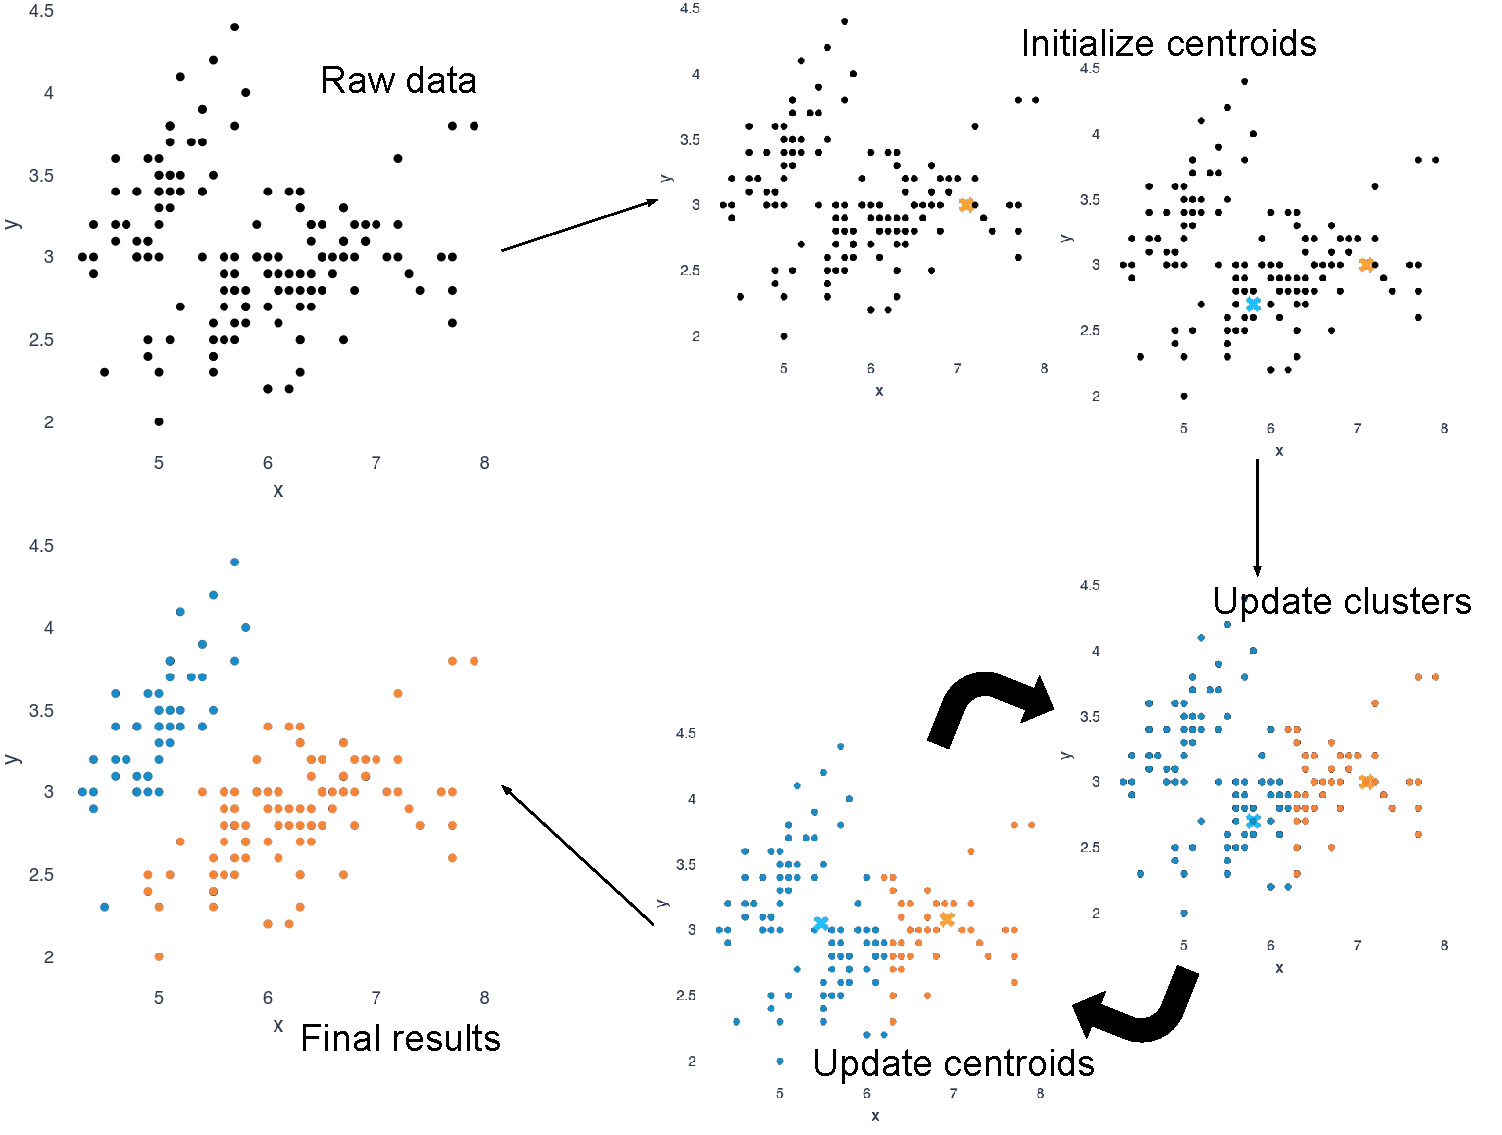
\includegraphics[width=\textwidth]{figures/410_method/kmeans/K-Means++ diagram.pdf}
%     \caption{\textbf{K-Means clustering.} The algorithm performs an iterative search by alternately grouping observations around cluster centers of mass and updating such centroids.}
%     \label{fig:kmeans-pipeline}
% \end{figure}

In this study, we resort to clustering for grouping messages including similar content.
The resulting clusters are therefore interpreted as error categories.
In particular, we adopt a slight variation of the above algorithm referred to as \mbox{\textbf{k-means++}} \cite{arthur2006kmeans++}.
The two techniques share the same workflow except for how the starting centroids are initialized.  
Specifically, the \mbox{k-means} algorithm assigns equal probability to all the data points and then samples $k$ centers.
For \mbox{k-means++} instead, only the first centroid is chosen uniformly at random. The following $k-1$ centers are sampled from data points with probability inversely proportional to the distance between each point and the closest predefined centroid.
This careful seeding strategy ensures the initial centers are more spread across the data points, thus favoring better clustering results and a faster convergence.
Despite more advanced clustering algorithms are available and may be applied to our use case, e.g. DBSCAN \cite{ester1996dbscan}, HDBSCAN \cite{mcinnes2017hdbscan}, BIRCH \cite{zhang1996birch}, OPTICS \cite{ankerst1999optics}, spectral clustering \cite{ng2002spectral} and so on, the choice of the a \mbox{k-means} algorithm is justified by its intuitive approach and good performance in practice in a wide range of applications \cite{von2012clustering}.
Also, a perhaps more profound and substantial motive is that the clustering strategy may be seen as a functional but not primary pipeline stage. Indeed, the learned language model determines the geometry of the embedded space, thus influencing the point cloud shapes of different error categories. 
For this reason, we embrace the idea that a simple clustering algorithm is preferable, and particular attention must be devoted to tuning the vectorization stage for easing the subsequent clustering, possibly even fostering the learning of an optimal representation for a specific clustering algorithm (\cite{yang2017kmeans-friendly}).

In order to demonstrate the approach, we report the analysis of FTS data from one full day of operation (2021-01-15), corresponding to roughly 1 M errors and 1.5 GB of data.
To help the successive evaluation phase, only transfers between Tier-0, Tier-1s and Tier-2s are considered in the analysis.
In practice, more hyper-parameter configurations are explored to test the effect of different choices.
The first set of investigations regards the measure of similarity adopted to form the clusters. 
In this respect, we tested two alternatives, cosine similarity and the euclidean distance.
The former consistently outperformed euclidean distance in all attempted experiments, 
both in terms of cluster geometrical properties and interpretability of the results.
% both considering clusters compactness and separation and in terms of interpretability of the results. 
For this reason, only the the analysis involving \textbf{consine similarity} is reported in the following.

Another crucial hyper-parameter is given by the assumed number of clusters, $k$. This represents the number of error categories in our case, which is not known in advance. 
Therefore a grid search for $k \in [12, 15, 20, 30] $ is exploited to retrieve a reasonable estimate from the data.
For this purpose, two geometrical criteria are considered to compare results of different settings, namely the \textit{Within cluster Sum of Squared Errors} (WSSE) and the \textit{Average Silhouette Width} (ASW) \cite{rousseeuw1987ASW}.
The WSSE measures the internal cluster variability, so the lower its value, the better the performance.
In terms of its definition, the WSSE is based on the total sum of squared distances between the points of each group and the correspondent centroid:
\begin{equation}
    \text{WSSE}\left(\text{dist}, k\right) = 
    \sum_{j=1}^{k}{ 
    \sum_{x_i \in C_j}{\text{dist}\left( x_i - \bar{x}_j\right)} 
    }
\end{equation}
where $x_i$ is a generic data point, ${dist}$ is a desired distance measure, and $C_j$ and $\bar{x}_j$ indicate a generic cluster and its centroid, respectively.
Although compactness is certainly a desirable property for the output groups, this metric is strongly affected by the scale of the variables and the number of observations. Indeed, the clusters exhibit a greater variability as their points present higher values and/or the cluster size increases, thus causing the WSSE to explode. 
Also, being unbounded by its nature, i.e. $\text{WSSE} \in \left[ 0, +\inf \right]$, the WSSE is of difficult interpretation on its own and it only makes sense when compared to other values. \\
% In fact, its absolute value have little sense on its own, and it only takes meaning when compared to other.
A better metric is the so-called average silhouette width. In brief, the ASW is a measure of clustering performance that accounts for both internal homogeneity and external separation of the clusters.
In particular, let $\bar{a}_i$ be the average distance of $x_i$ from all the other points belonging to the same cluster $C_I$. Also, let $b_i$ be the minimum average distance of $x_i$ from the observations in all the other clusters $C_j , \forall j \neq I$. Then, the ASW is defined as:
\begin{equation}
    \text{ASW}\left(\text{dist}, k\right) = 
    \dfrac{1}{n} \sum_{i=1}^{n}{ 
    \dfrac{b_i - \bar{a}_i}{ max\left( \bar{a}_i, b_i \right) }
    }
\end{equation}
where $n$ is the total number of observations, i.e. error messages in our case.
The average silhouette is much more intuitive to interpret than the WSSE as its value is bounded in the interval $\left[ -1, +1 \right]$.
In practice, negative values of the ASW mean that points of one cluster are on average more similar to observations of other groups than the ones of their own cluster. A value of 0, instead, suggest that the groups are not really distinguishable, thus making the assignation of single observations to any of the clusters arbitrary.
Finally, positive values close to 1 testify that the clustering produces nicely homogeneous groups that are also well separated.
Given the more intuitive reading of ASW values, the latter is used in the following as the main figure of merit.

% Apart from the distance and the value of $k$, the other hyper-parameters were not optimized and the values \textbox{initSteps=200}, \textbox{tol=0.0001}, \textbox{maxIter=100} were chosen.

The results of the comparison between WSSE and ASW for different values of $k$ are reported in \cref{fig:k_optim}.
Both indicators tend to improve as the number of clusters increases.
In particular, a value of $k=30$ clusters seems to be optimal according to both criteria.
Notably, however, the ASW indicator reaches very high values (around 0.9) even for lower $k$ values.
% of 0.9405 which is a very high score for this metric.
For this reason, the configuration having $\boldsymbol{k=15}$ is preferred to limit the number of suggested issues and minimize the shifters effort.
% considered for the discussion in \cref{ch:opint-results}. 

\begin{figure}
    \centering
    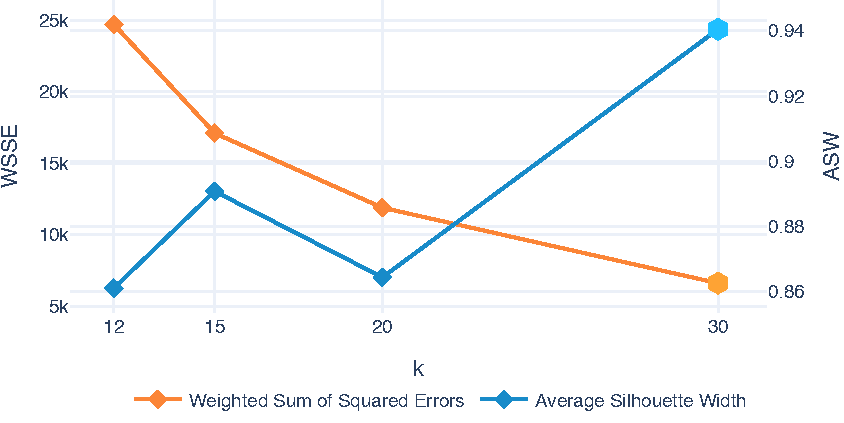
\includegraphics[width=\textwidth]{figures/410_method/kmeans/k_optim.pdf}
    \caption{\textbf{Optimization of $\boldsymbol{k}$.} The plot shows the value of the WSSE and ASW metrics as a function of the number of clusters $k$. The hexagonal markers indicate the optimal values, which correspond to $k=30$ for both indicators.}
    \label{fig:k_optim}
\end{figure}

\subsection{Cluster description}\label{sec:viz}

% The last stage of the pipeline is cluster description. 
% This step is fundamental to present the results in the most intelligible and concise format for the end-users to consume it.

% Once we have clusters of data, the next step is to inspect their content to try to grasp their meaning.
% Given the unsupervised learning approach adopted, this interpretation phase is troublesome and time-demanding.

% In order to demonstrate the approach, we report an analysis of FTS data from one full day of operation. %(15/01/2021).

The last stage of the pipeline is cluster description. 
This step is fundamental to present the results in the most intelligible and immediate format for end-users.
Indeed, given the unsupervised learning approach adopted, the interpretation of the clustering output resorts to the manual inspection of each group's content.
This, in turn, potentially mean reading hundreds of error strings, comparing the source and destination information, and spotting suspect time patterns.  
%This implies a troublesome and time-demanding evaluation phase, which partly balances the effort saved by avoiding the collection of a reference dataset of known issues and corresponding solutions.
Therefore, producing a nice and compact visualization of the results is paramount to make the approach effective and avoid excessive manual checks by the operators.
For this reason, the clustering results are summarized into two complementary outputs that are presented to the shifters.

First, the \textit{summary table} represents the most important and informative visualization.
This output is obtained by a first pre-aggregation of the clusters and is organized in a tabular format.
The first three columns provide numeric summaries concerning the  cluster size, the number of unique strings within each group, and the corresponding number of unique patterns.
The latter is obtained from the raw strings by means of an \textit{abstraction mechanism}\footnote{refer to the full implementation for more details: \githubabstractions} that removes the parametric parts -- like file paths, IP addresses, URLs, checksum values, and so on -- and replaces them by parameter-specific placeholders -- e.g. \textbox{\$FILE\_PATH}, \textbox{\$ADDRESS}, \textbox{\$URL} and  \textbox{\$CHECKSUM}, respectively.
The core part of this visualization is then represented by the \textit{Top 3} section. Here, the three most frequent triplets of \textbox{<pattern>-<source>-<destination>} are reported in descending order for each cluster, alongside their cardinality and the percentage over the cluster size.
Such information provides several precious insights for spotting the source of potential problems, e.g. whether a pattern is responsible for a large number of failures or if it accounts for a conspicuous fraction of the cluster. 
In addition, this representation allows us to investigate the contribution of source/destination pairs to each cluster.
In this way, it is possible to discriminate failures based on both the nature of the problem and the location where they occurred.
An example of summary table is reported in \cref{fig:cluster_summary:successes,fig:cluster_summary:failures}.
% \Cref{fig:cluster0} shows an example of summary table for the biggest cluster found in the analyzed period.

The second output of the pipeline consists of a time-series chart depicting the temporal evolution of the number of errors generated by each cluster
(\cref{fig:timeplots}).
% (\cref{fig:timeplot_cluster0}).
This piece of information is crucial to discriminate between serious issues that require immediate actions (\cref{fig:timeplots:growing,fig:timeplots:cyclical}) and transient (\cref{fig:timeplots:transient}) problems. 

Overall, the idea behind our pipeline is to exploit the summary tables and the time plots for each cluster as suggestions of potential issues to investigate further.
In this way, the shifters can have a first grasp of what kind of failures are observed and their corresponding amounts (Top-3 section), also having an indication of where they are happening (source/destination sites).
Moreover, by looking at the time charts it is possible to immediately discard transient (\cref{fig:timeplots:transient}) or resolved (\cref{fig:timeplots:resolved}) problems based on the evolution of the number of generated failures over time.


% \begin{figure}
%     \centering
%     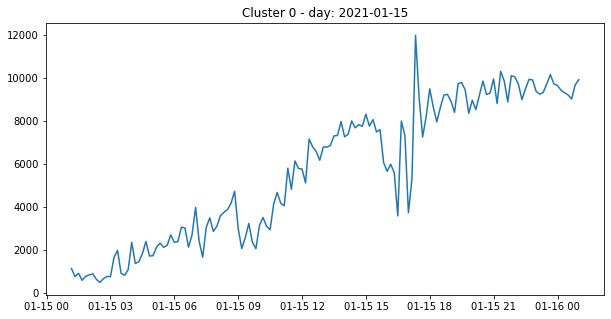
\includegraphics[width=\textwidth]{figures/510_results/timeplot_cluster0.png}
%     \caption{\textbf{Time evolution of cluster 0}. The plot shows the count of errors in bins of 10 minutes.}
%     \label{fig:timeplot_cluster0}
% \end{figure}

\begin{figure}
    \centering
    \subfloat[growing]{
    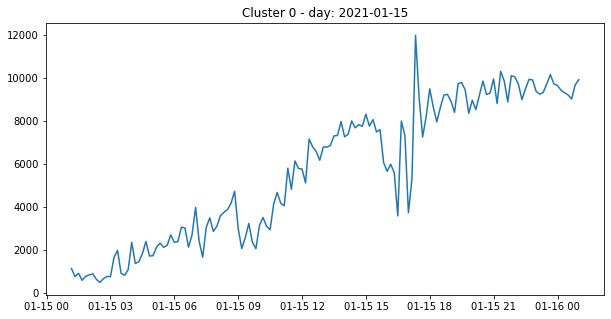
\includegraphics[width=0.5\textwidth]{figures/510_results/timeplots/cluster_0.png}\label{fig:timeplots:growing}
    \label{fig:timeplots:growing}
    }
    \subfloat[transient]{
    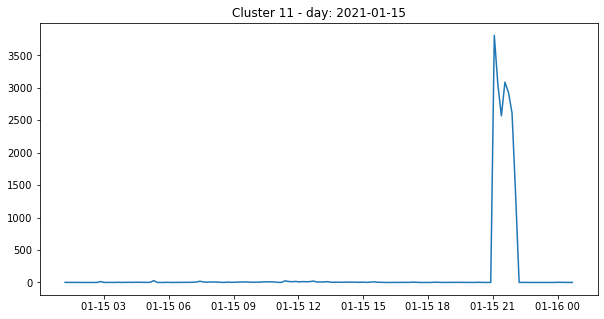
\includegraphics[width=0.5\textwidth]{figures/510_results/timeplots/cluster_11.png}\label{fig:timeplots:transient}
    \label{fig:timeplots:transient}
    }
    
    \subfloat[resolved]{
    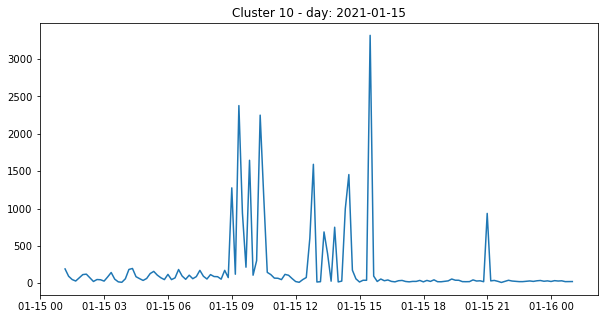
\includegraphics[width=0.5\textwidth]{figures/510_results/timeplots/cluster_10.png}\label{fig:timeplots:resolved}
    }
    \subfloat[cyclical]{
    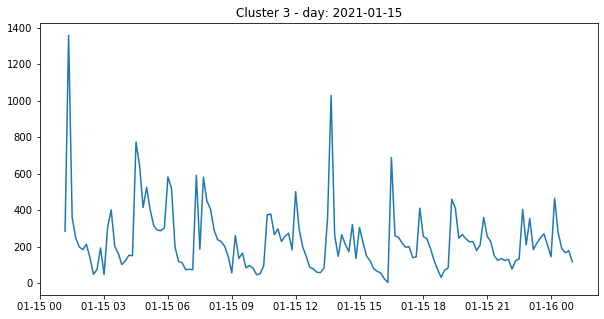
\includegraphics[width=0.5\textwidth]{figures/510_results/timeplots/cluster_3.png}\label{fig:timeplots:cyclical}
    }
    \caption{\textbf{Time evolution charts}. The figure illustrates several time patterns for the generated failures in 4 different clusters. Each plot reports the count of errors in bins of 10 minutes.}
    \label{fig:timeplots}
\end{figure}